\documentclass[11pt,a4paper]{article}
\usepackage[margin=2.25cm]{geometry}
\usepackage[T1]{fontenc}
\usepackage[utf8]{inputenc}
\usepackage{lmodern,microtype,amsmath,amssymb,graphicx,booktabs,array,caption,float}
\usepackage[dvipsnames]{xcolor}
\usepackage[colorlinks=true,linkcolor=MidnightBlue,citecolor=MidnightBlue,urlcolor=MidnightBlue]{hyperref}
\usepackage{fancyhdr}
\hypersetup{pdftitle={Revisiting GW190521 with open data: waveform timing, noise weighting and network consistency},pdfauthor={Hemendra Singh}}
\graphicspath{{../figures/}{figures/}}
\pagestyle{fancy}\fancyhf{}\fancyhead[L]{\small GW190521: an open data methods study}\fancyhead[R]{\small H. Singh}\fancyfoot[C]{\thepage}
\setlength{\headheight}{14pt}
\setlength{\parindent}{0pt}\setlength{\parskip}{3pt}
\captionsetup{font=small,labelfont=bf}
\newcommand{\Msun}{M_{\odot}}
\title{\vspace{-1.3cm}Revisiting GW190521 with open data:\\waveform timing, noise weighting\\and network consistency}
\author{Hemendra Singh\\\small Gravity Exploration Institute\\\small School of Physics and Astronomy, Cardiff University\\\small Work carried out in 2024}
\date{Revised 3 October 2026\\\small Methods note accompanying software version 0.2.2}
\begin{document}
\maketitle
\begin{abstract}
The short duration of GW190521 makes it a useful case for examining how implementation choices affect a comparison between physical and phenomenological gravitational wave templates. This study presents a reproducible analysis of public Hanford, Livingston and Virgo strain, using quality screened off-source noise estimates, explicit waveform reference times and three separately defined network statistics. Two nonspinning compact binary templates are compared with a circularly polarised sine Gaussian, evaluated both at a fixed shape and on a declared frequency and quality-factor grid. The common-time quadrature statistic is 14.175 for the fixed sine Gaussian, 14.481 for \texttt{SEOBNRv4\_opt} and 13.949 for \texttt{IMRPhenomXPHM}; the best sampled sine Gaussian reaches 14.466. A controlled ablation shows that discarding the burst template's reference time reduces its independent-peak summary from 14.314 to 5.682. Independent time-domain injections and Gaussian-noise amplitude tests validate the corrected conventions. These results describe a restricted morphology comparison and a reproducibility case study. They do not provide source-parameter posteriors, detection significance or evidence favouring one astrophysical interpretation.
\end{abstract}

\section{Scientific purpose and scope}
GW190521 was reported as a short gravitational wave signal consistent with the merger of two massive black holes \cite{discovery,implications}. Its observable structure occupies only a few cycles at frequencies of tens of hertz. Such a signal motivates comparisons between compact binary coalescence (CBC) waveforms and simpler localised oscillations. It also makes timing conventions particularly consequential: shifting a short template outside the selected event interval can look like a failure of the signal model.

The starting point for this work was an MSc analysis notebook, subsequently reconstructed as reusable software. The present study asks a deliberately limited question: \emph{what can a consistently conditioned, timing-validated comparison of fixed waveform shapes establish about the recovery of GW190521?} The analysis is designed to make its numerical results inspectable, including the detector responses, accepted noise windows, exact statistic definitions and limitations.

The two CBC templates use the same illustrative masses, distance and orientation, with all spins fixed to zero. The burst model is tested at one specified shape and over a bounded grid. Consequently, this is not a controlled measurement of the effect of precession or higher modes. Nor does a maximum filter statistic on this grid constitute Bayesian model selection. Throughout, ``recovery'' refers to a filtering statistic, not recovery of the source's astrophysical parameters.

\section{Data, quality selection and noise estimation}
\subsection{Public strain and analysis intervals}
The input is the GWOSC GWTC 2.1 version 4 event release \cite{data,opendata}. The analysis downloads the three 4096 s, 4096 Hz HDF5 records for H1, L1 and V1. Their common start time is GPS 1242440920. The catalogue event reference is GPS 1242442967.4. SHA-256 hashes and original download addresses are recorded in the machine-readable analysis metadata; the raw strain is excluded from the software distribution.

The time series are resampled to 2048 Hz after reading an interval with additional boundary padding. The event segment is GPS $[1242442951,1242442983)$, with a one-second Tukey taper at each boundary and its mean removed. Filtering uses the original strain and a noise PSD. Whitened, bandpassed strain is used only for visualisation. This avoids applying whitening twice in the matched filter.

\begin{table}[ht]
\centering\small
\begin{tabular}{ll}
\toprule
Choice & Value \\
\midrule
Event segment & 32 s \\
Off-source PSD interval & GPS $[1242442423,1242442935)$ \\
Separation from catalogue event time & 32.4 s after the end of the PSD interval \\
PSD periodograms & 8 s Hann windows, 4 s stride \\
PSD aggregation & Median with finite-sample median bias correction \\
Analysis frequency interval & $20\leq f<256$ Hz \\
On-source reference-time interval & Catalogue GPS $\pm0.15$ s \\
SNR boundary exclusion & 4 s at each end \\
\bottomrule
\end{tabular}
\caption{Default settings. All detectors share the same filtering band and reference-time search interval.}
\end{table}

\subsection{Quality flags and the off-source PSD}
The event segment passes the available DATA, CBC CAT1/CAT2 and BURST CAT1/CAT2 flags, and the no-CBC and no-burst hardware-injection flags, in all three detectors. The initial 512 s noise interval contains seconds failing BURST CAT2. Rather than treating the full interval as uniformly usable, every candidate 8 s PSD window is checked against the same flags, with a one-second guard on both sides. A window touching a veto is excluded.

Of 127 candidate windows, 124 are retained for H1, 108 for L1 and 127 for V1. Each accepted periodogram uses constant detrending and a Hann window. The frequency-wise median is divided by PyCBC's finite-sample median-bias factor. The resulting PSD has a native frequency spacing of 0.125 Hz and is interpolated to the event Fourier grid, whose spacing is 0.03125 Hz. The usual median correction is used; no additional correction for correlations between overlapping windows is applied.

This procedure is robust to some isolated contamination, but it does not establish Gaussianity or stationarity of the noise \cite{noise}. PSD uncertainty is not marginalised. A shorter, quality screened 256 s noise interval is therefore included as a sensitivity check. The same default PSDs are supplied to whitening and to the descriptive Q transforms, implemented with GWPy \cite{gwpy}.

\begin{figure}[ht]
\centering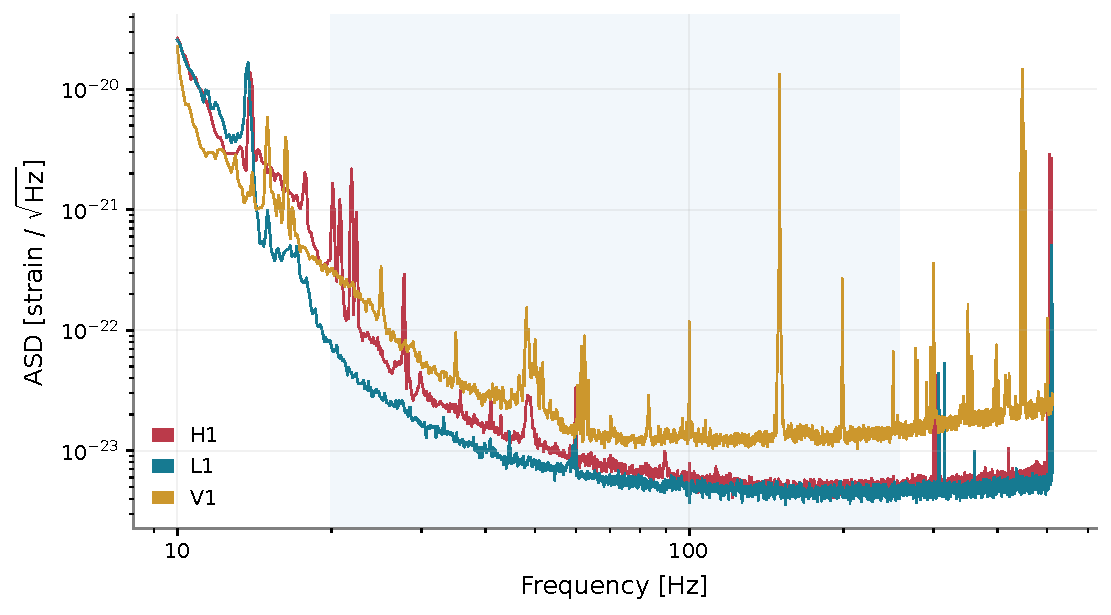
\includegraphics[width=.83\linewidth]{detector_psd.pdf}
\caption{Off-source amplitude spectral densities after quality screening. The shaded interval is the common filtering band.}
\end{figure}

\section{Signal models and reference-time conventions}
\subsection{Fixed compact binary templates}
The illustrative source-frame inputs are $m_1=98.4\,\Msun$, $m_2=57.2\,\Msun$, $z=0.56$ and luminosity distance $d_L=3310$ Mpc, taken from the displayed marginal summaries of the selected GWOSC release \cite{data}. The waveform masses are
\begin{equation}
 m_i^{\mathrm{det}}=(1+z)m_i^{\mathrm{source}},
\end{equation}
which gives $153.504\,\Msun$ and $89.232\,\Msun$. A vector assembled from marginal summaries is not a joint posterior sample or a maximum-likelihood solution. These inputs are a documented reference point, not newly inferred values. PyCBC's luminosity-distance convention is Mpc.

The \texttt{SEOBNRv4\_opt} waveform is generated in the time domain and tapered at its beginning; \texttt{IMRPhenomXPHM} is generated in the frequency domain \cite{seobnr,phenom,pycbc}. Both start at 15 Hz, below the 20 Hz filtering threshold. The frequency-domain reference frequency is 20 Hz. All component spins and the reference coalescence phase are zero. The inclination is 1.0 rad. Although the latter waveform family supports precession and higher harmonics, the configuration here has no spin-induced precession. Differences between these two waveforms cannot be assigned solely to their harmonic content.

\subsection{Sine Gaussian and the exploratory grid}
The burst model has polarisations
\begin{align}
 h_+(t)&=A\exp\left[-\frac{t^2}{2\sigma_t^2}\right]\cos(2\pi f_0t),\\
 h_\times(t)&=\epsilon A\exp\left[-\frac{t^2}{2\sigma_t^2}\right]\sin(2\pi f_0t),
 \qquad Q=2\pi f_0\sigma_t.
\end{align}
The default choices are $f_0=60$ Hz, $Q=8$ and $\epsilon=1$. The last choice is circular polarisation, a particular case of elliptical polarisation. Both polarisations are nonzero. The arbitrary amplitude $A=10^{-21}$ cancels from normalised single-detector filtering and is not a fitted strain amplitude.

An exploratory grid contains frequencies from 40 to 90 Hz in 2 Hz increments and integer $Q$ from 2 to 20, giving 494 shapes. The largest common-time quadrature statistic selects a grid point at $f_0=58$ Hz and $Q=6$. This is a discrete optimisation of morphology on the observed event. It is not a posterior credible region. The grid was not preregistered, and its maximisation introduces a trials effect that is not converted into a significance claim.

\subsection{Detector projection and physical time}
For each detector $I$, both polarisations are projected as
\begin{equation}
 \widetilde h_I(f)=\left[F_I^+\widetilde h_+(f)+F_I^\times\widetilde h_\times(f)\right]
 e^{-2\pi i f\Delta t_I}.
\end{equation}
The antenna factors and Earth-centre delays are evaluated at the catalogue GPS time. The illustrative geometry is right ascension 3.6 rad, declination $-0.7$ rad and polarisation angle 1.5 rad. It is held fixed and is not a sky localisation result. The delays are approximately $+1.484$ ms (H1), $-6.739$ ms (L1) and $+9.068$ ms (V1).

A sampled time-domain template has a physical start time $t_s$ relative to its geocentric reference. An FFT of its array alone treats the first sample as time zero. After padding to the event duration, the correct reference spectrum is
\begin{equation}
 \widetilde h_{\rm ref}(f_k)=\widetilde h_{\rm array}(f_k)e^{-2\pi i f_kt_s}.
 \label{eq:epoch}
\end{equation}
For a centred four-second burst, neglecting this factor introduces an approximately two-second reference error. Merely attaching an epoch to an array is insufficient if a subsequent filter does not use that epoch in its Fourier phase. Equation~\ref{eq:epoch} includes the detector delay for the time-domain templates; the delay is applied explicitly for the frequency-domain template. Filter outputs can then be evaluated on one geocentric reference-time grid.

\section{Noise-weighted comparisons and network statistics}
The discrete one-sided inner product is
\begin{equation}
 (a|b)_I=4\,\Delta f\,\mathrm{Re}\sum_{20\leq f_k<256\,\mathrm{Hz}}
 \frac{\widetilde a(f_k)^*\widetilde b(f_k)}{S_I(f_k)}.
\end{equation}
Let $\sigma_I^2=(h_I|h_I)_I$ and let $z_I(t)$ denote the complex, normalised matched-filter output. Its magnitude maximises over a filter quadrature phase. A waveform match is the normalised noise-weighted inner product maximised over relative time and quadrature phase. This phase maximisation is a mathematical filter operation; for a multimode waveform it need not equal variation of one physical orbital phase.

Three network quantities are retained because they answer different questions:
\begin{align}
 \rho_{\rm bound}&=\left[\sum_I\max_{t\in W}|z_I(t)|^2\right]^{1/2},\\
 \rho_{\rm time}&=\max_{t\in W}\left[\sum_I|z_I(t)|^2\right]^{1/2},\\
 \rho_{\rm fixed}&=\max_{t\in W}
 \frac{\left|\sum_I\sigma_I z_I(t)\right|}{\left[\sum_I\sigma_I^2\right]^{1/2}},
 \label{eq:coherent}
\end{align}
where $W$ is the declared on-source interval. The first combines independent detector maxima and is an upper bound, not a coincidence test. The second imposes a common geocentric reference time while retaining independent detector amplitudes and phases. The third retains the prescribed relative detector responses and profiles over one common complex coefficient. It is a coherent projection onto the fixed network template, rather than a search over physical source parameters. They satisfy
$\rho_{\rm fixed}\leq\rho_{\rm time}\leq\rho_{\rm bound}$.

For independent Gaussian detector noise, the implemented log likelihood ratio for an already aligned network waveform is
\begin{equation}
 \log\frac{\mathcal L(d|h)}{\mathcal L(d|0)}=
 \sum_I\left[(d_I|h_I)_I-\tfrac12(h_I|h_I)_I\right].
\end{equation}
Profiling a common complex coefficient produces $\rho_{\rm fixed}^2/2$. This construction includes coherent detector amplitudes, phases and delays, but does not integrate over them. No prior or Bayesian evidence is used. Introducing astrophysical priors without actually performing inference would not turn these filter statistics into posteriors.

\section{Results and validation}
\subsection{Recovered statistics and shape similarity}
\begin{table}[ht]
\centering\small\setlength{\tabcolsep}{4pt}
\begin{tabular}{lrrrrrr}
\toprule
Template & H1 & L1 & V1 & $\rho_{\rm bound}$ & $\rho_{\rm time}$ & $\rho_{\rm fixed}$\\
\midrule
% BEGIN GENERATED RESULTS
Sine Gaussian, fixed & 7.849 & 11.315 & 3.906 & 14.314 & 14.175 & 6.862 \\
\texttt{SEOBNRv4\_opt} & 8.699 & 11.535 & 3.544 & 14.876 & 14.481 & 8.487 \\
\texttt{IMRPhenomXPHM} & 8.179 & 10.960 & 3.712 & 14.170 & 13.949 & 8.301 \\
Sine Gaussian, grid & 7.933 & 11.741 & 3.682 & 14.640 & 14.466 & 7.743 \\
% END GENERATED RESULTS
\bottomrule
\end{tabular}
\caption{The first three columns are independently maximised single-detector filter magnitudes. Network columns use the distinct definitions above. The grid burst is selected using $\rho_{\rm time}$, so it has more freedom than the fixed templates.}
\label{tab:snr}
\end{table}

Both the fixed burst and the CBC templates give common-time statistics near 14. A short sine Gaussian therefore captures much of the observed signal's morphology under this restricted comparison. The best grid value is close to the \texttt{SEOBNRv4\_opt} reference, but this proximity does not establish equal astrophysical plausibility. The grid has been optimised on the data, whereas the CBC source parameters have not.

With H1 PSD weighting, the two CBC templates have a match of 0.961. The fixed burst matches \texttt{SEOBNRv4\_opt} and \texttt{IMRPhenomXPHM} at 0.804 and 0.786, respectively; the grid burst gives 0.854 and 0.838. These quantify pairwise shape similarity at the selected parameters. Matches for each detector are supplied in the release, since the weighting depends on its noise spectrum.

\begin{figure}[ht]
\centering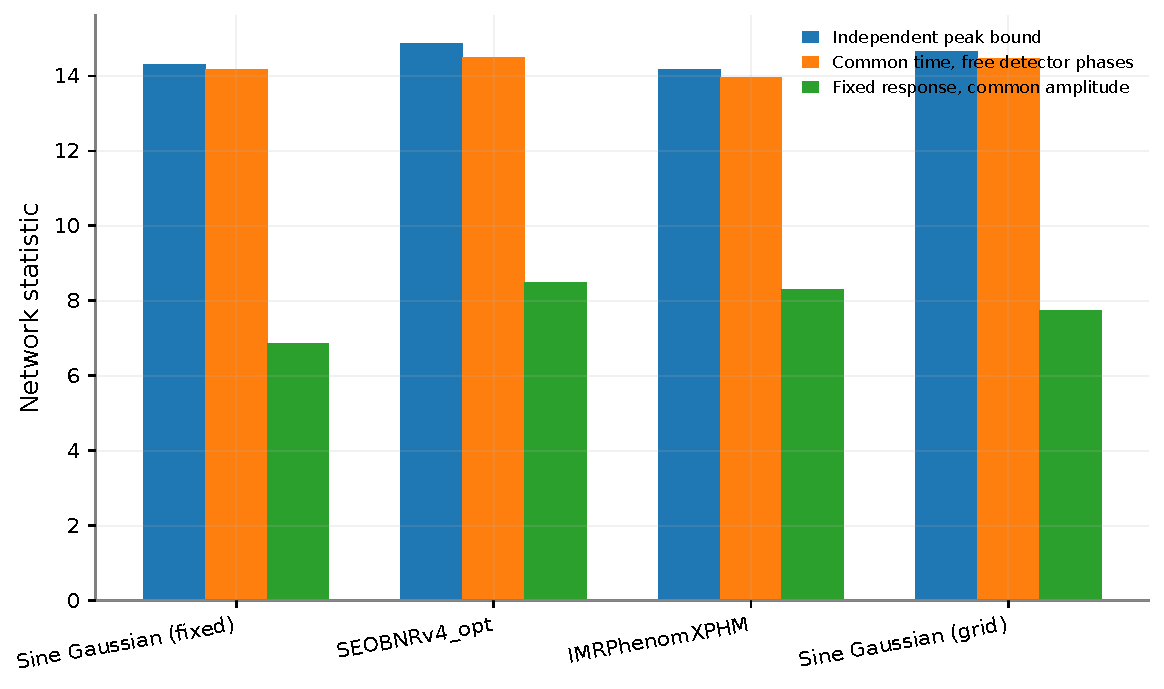
\includegraphics[width=.94\linewidth]{snr_comparison.pdf}
\caption{Separating independent maxima, common-time quadrature and fixed-response coherence exposes the assumptions hidden by a single ``network SNR'' label.}
\end{figure}

The fixed-response values are much smaller than the quadrature values. The geometry and polarisation are illustrative rather than fitted, so their amplitude and phase relations need not match the data. These numbers must not be interpreted as evidence that the observed event is incoherent. They show the cost of imposing this particular response. A physical joint analysis would explore the allowed sky, orientation, phase and intrinsic parameters.

The selected GWOSC release reports a parameter-estimation network matched-filter SNR of $14.3^{+0.5}_{-0.4}$, with different search pipelines reporting other values \cite{data}. It is useful as a scale reference only. Agreement with that number is not an independent validation because the pipelines, signal parameters, response treatment and noise assumptions differ.

\begin{figure}[ht]
\centering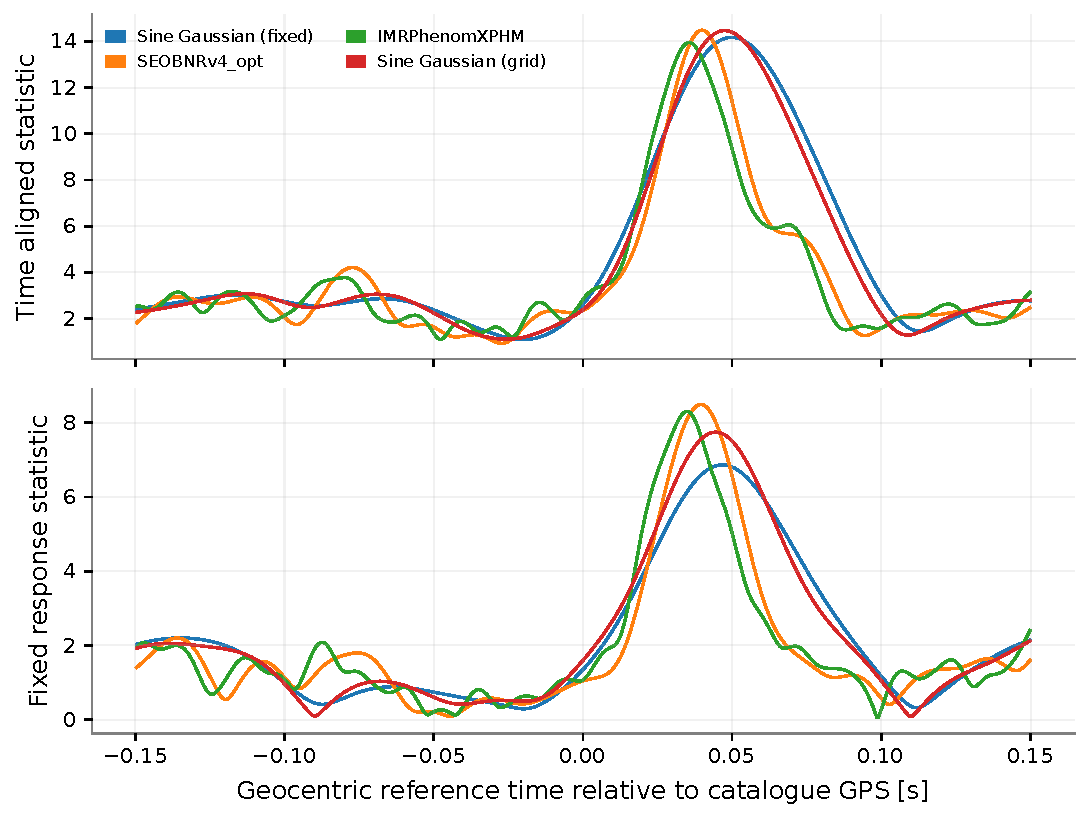
\includegraphics[width=.88\linewidth]{network_timeseries.pdf}
\caption{The reference time is geocentric in both panels. Peaks from different waveform shapes need not coincide exactly because their reference phase and morphology differ.}
\end{figure}

\subsection{An isolated reference-time ablation}
A controlled test keeps the new burst shape, data, PSD and analysis band unchanged, but discards the time-domain template epoch before filtering. The independent-peak summary decreases from 14.314 to 5.682, while the common-time statistic decreases from 14.175 to 4.404. Restoring the physical Fourier phase restores the event recovery. Thus the previous low burst recovery was dominated by an implementation error; it cannot support a claim that this burst shape fails to recover GW190521.

This ablation is not a reconstruction of every setting in the earlier software, whose quality-factor and PSD conventions also differed. Its purpose is to isolate the timing error under one fixed, reproducible configuration. The previous release's burst SNR and conclusions based on it are superseded.

\subsection{Independent injections and noise normalisation}
Eleven regression cases check mass conventions, physical arrival times, frequency-domain delays, invariance to zero padding, network-statistic ordering and the likelihood normalisation. For each detector, an analytic burst is evaluated directly on the injection time grid, independently of the template's FFT reference conversion. Separate CBC tests place the time-domain waveform by interpolation. The recovered geocentric times agree with the injected reference to within one sample, $1/2048$ s.

For a noise test, each of the three fixed waveform shapes is injected at an optimal network SNR of 20 into 128 independent Gaussian-noise realisations generated from the measured detector PSDs. The shape, time, phase and geometry are assumed known. The only recovered quantity is one real network amplitude, whose expected standard deviation is $1/20$. If $A_0=1$, the standardised error is $u=20(\widehat A-A_0)$.

\begin{table}[ht]
\centering\small
\begin{tabular}{lrrrr}
\toprule
Template & Mean $u$ & Sample SD $u$ & $|u|\leq1$ & $|u|\leq2$\\
\midrule
Sine Gaussian & 0.021 & 0.925 & 0.719 & 0.977\\
\texttt{SEOBNRv4\_opt} & $-0.050$ & 0.971 & 0.688 & 0.945\\
\texttt{IMRPhenomXPHM} & $-0.020$ & 1.009 & 0.633 & 0.969\\
\bottomrule
\end{tabular}
\caption{Conditional amplitude checks in synthetic noise; 128 draws per row, random seed 20261002. The expected mean and standard deviation are zero and one. The fractions have finite-sample uncertainty and do not test astrophysical posterior coverage.}
\end{table}

These results are consistent with the expected likelihood normalisation at this sample size. They validate neither waveform accuracy nor recovery of masses, spins, distance or sky position in real, nonstationary noise. The CBC and frequency-domain injections also reuse the waveform generator, so they cannot reveal errors shared with that generator.

\subsection{Dependence on frequency band and PSD interval}
The release repeats the filtering with bands of 20 to 128 Hz, 25 to 256 Hz and 30 to 256 Hz, and with the nearest quality screened 256 s PSD interval. Template parameters are held fixed, including the burst grid selection. Across these checks, $\rho_{\rm time}$ ranges from 14.047 to 14.175 for the fixed burst, 14.353 to 14.573 for \texttt{SEOBNRv4\_opt}, 13.801 to 14.014 for \texttt{IMRPhenomXPHM}, and 14.305 to 14.468 for the selected burst. The similarity in recovery scale survives these choices. This limited sensitivity study does not sample all plausible conditioning choices or quantify a systematic uncertainty.

\section{Interpretation and remaining scientific work}
The practical outcome is a comparison with explicit assumptions and a demonstrated correction to template timing. A sine Gaussian can recover a substantial fraction of the filtering response of this short event without describing a complete binary merger. Conversely, a high template match or a plausible SNR does not establish an astrophysical measurement. Parameter choices, detector weighting, timing and coherence must all be distinguished.

This study does not infer the component masses, luminosity distance or redshift; the displayed values are inputs. It does not establish precession, measure higher-mode content or rank eccentric, lensed, hierarchical-merger or other interpretations. The use of a more flexible waveform family at zero spin cannot supply those conclusions.

A source-inference extension would require a physical network likelihood over intrinsic and extrinsic parameters, finite documented priors, posterior exploration with convergence diagnostics, injection studies spanning the claimed parameter region and comparison with the released joint posterior samples under matched conventions. Calibration uncertainty, PSD uncertainty and the sensitivity to nonstationary transients would also need treatment. Any model-selection comparison must account for different parameter volumes and the burst search's additional freedom. None of those unperformed analyses is replaced here by a short MCMC run or by an optimiser's best point.

The current output is therefore a reproducible methods and software contribution with a narrow claim. Its value is the inspectable connection between code conventions and recovered statistics. Independent scientific review should assess its archival contribution before a preprint submission presents it as a research result beyond that scope.

\section{Reproducibility, provenance and acknowledgements}
The companion project contains importable source code, a runnable notebook, an HTML rendering, tests, exact numerical tables, vector figures, data-quality accounting, checksums and a pinned environment snapshot. Running the analysis regenerates the main tables and figures; a separate script regenerates the amplitude tests. The repository's documentation gives the commands and distinguishes completed validation from future work.

The work was carried out in 2024 at the Gravity Exploration Institute, School of Physics and Astronomy, Cardiff University. The public implementation and methods note were subsequently reconstructed and revised from that project. The original coursework instructions are not redistributed. The reported checks are computational checks, not independent peer review.

The analysis uses public data and software from the Gravitational Wave Open Science Center, supported by the LIGO Scientific Collaboration, Virgo and KAGRA. The selected data release is licensed under CC BY 4.0 \cite{data}; the analysis code uses the BSD 3-Clause licence. PyCBC, LALSuite, GWPy, NumPy, SciPy, Astropy, pandas and Matplotlib provide the numerical and visualisation infrastructure. Their exact versions are recorded with the results. No new detector data were collected for this study.

\begin{thebibliography}{10}\small
\bibitem{discovery} R. Abbott et al. (LIGO Scientific Collaboration and Virgo Collaboration), ``GW190521: A Binary Black Hole Merger with a Total Mass of $150\,M_\odot$'', \emph{Physical Review Letters} \textbf{125}, 101102 (2020). \href{https://doi.org/10.1103/PhysRevLett.125.101102}{doi:10.1103/PhysRevLett.125.101102}.
\bibitem{implications} R. Abbott et al., ``Properties and astrophysical implications of the 150 $M_\odot$ binary black hole merger GW190521'', \emph{Astrophysical Journal Letters} \textbf{900}, L13 (2020). \href{https://doi.org/10.3847/2041-8213/aba493}{doi:10.3847/2041-8213/aba493}.
\bibitem{data} GWOSC, ``GW190521, GWTC-2.1-confident, version 4'', event strain and parameter summary. \href{https://gwosc.org/eventapi/html/GWTC-2.1-confident/GW190521/v4/}{Event release}; data DOI \href{https://doi.org/10.7935/qf3a-3z67}{10.7935/qf3a-3z67}. Accessed 2 October 2026.
\bibitem{opendata} R. Abbott et al., ``Open data from the third observing run of LIGO, Virgo, KAGRA and GEO, \emph{Astrophysical Journal Supplement Series} 	extbf{267}, 29 (2023). \href{https://doi.org/10.3847/1538-4365/acdc9f}{doi:10.3847/1538-4365/acdc9f}.
\bibitem{noise} B. P. Abbott et al., ``A guide to LIGO-Virgo detector noise and extraction of transient gravitational-wave signals'' (2020). \href{https://arxiv.org/abs/1908.11170}{arXiv:1908.11170}.
\bibitem{pycbc} S. A. Usman et al., ``The PyCBC search for gravitational waves from compact binary coalescence'' (2016). \href{https://arxiv.org/abs/1508.02357}{arXiv:1508.02357}; \href{https://pycbc.org/pycbc/latest/html/pycbc.filter.html}{PyCBC filtering documentation}.
\bibitem{seobnr} A. Boh\'e et al., ``An improved effective-one-body model of spinning, nonprecessing binary black holes for the era of gravitational-wave astrophysics with advanced detectors'' (2017). \href{https://arxiv.org/abs/1611.03703}{arXiv:1611.03703}.
\bibitem{phenom} G. Pratten et al., ``Computationally efficient models for the dominant and sub-dominant harmonic modes of precessing binary black holes'' (2021). \href{https://arxiv.org/abs/2004.06503}{arXiv:2004.06503}.
\bibitem{gwpy} D. M. Macleod et al., ``GWpy: A Python package for gravitational-wave astrophysics'', \emph{SoftwareX} \textbf{13}, 100657 (2021). \href{https://doi.org/10.1016/j.softx.2021.100657}{doi:10.1016/j.softx.2021.100657}.
\end{thebibliography}
\end{document}
